\newpage
\section{El problema}\label{sec:problema}

Un yacimiento petrol\'\i fero es una acumulaci\'on natural de hidrocarburos (gas natural y petr\'oleo, entre otros) en el subsuelo. Debido a la creciente escasez de reservas de hidrocarburos acumulados en yacimientos convencionales, la industria del petr\'oleo y diversos gobiernos nacionales han tornado su atenci\'on en las \'ultimas d\'ecadas a la explotaci\'on de yacimientos no convencionales. Uno de los tipos de yacimientos m\'as explorados est\'a dado por las reservas de petr\'oleo y gas natural almacenados en un tipo de rocas sedimentarias llamadas pelitas (shale), conocidos como yacimientos de \emph{shale gas} y \emph{shale oil}.
 
La explotaci\'on de este tipo de yacimientos utiliza m\'etodos de fractura hidr\'aulica, por medio de los cuales se generan fracturas en la roca madre para concentrar el petr\'oleo y el gas natural y posteriormente proceder a su extracci\'on. A pesar de que las primeras inyecciones de material para la extracci\'on de hidrocarburos se remontan a la segunda mitad del siglo XIX, reci\'en se comenz\'o a usar este tipo de m\'etodos en forma extensiva a prin\-ci\-pios del siglo XXI, principalmente en Estados Unidos. Adem\'as de las reservas en Estados Unidos, en la \'ultima d\'ecada se han descubierto enormes reservas de shale gas y shale oil en Argentina, Canad\'a y China.

Se describe el proceso de explotaci\'on de un yacimiento \emph{shale}. En primer lugar, se realizan varias perforaciones verticales en el subsuelo que llegan hasta la roca madre. Como se ve a continuacion:

\begin{center}
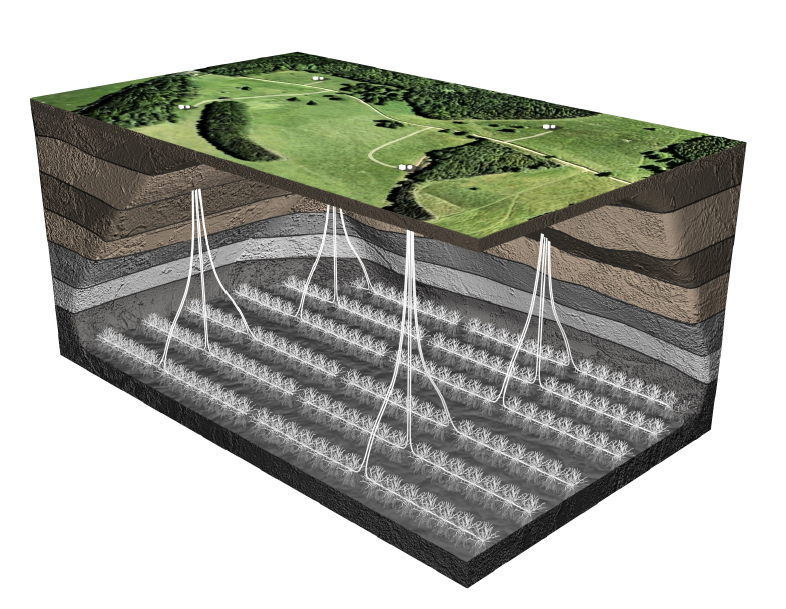
\includegraphics[width=0.15\textwidth]{imagenes/figura1}
\end{center}


El sector en la superficie alrededor de las bocas de pozo se denomina locacion, y habitualmente ocupa un area rectangular de entre algunas decenas y unos pocos cientos de metros por lado. Estos equipos son los unicos que se ven en la supercie, y habitualmente su instalacion involucra obras de nivelacion del suelo y construccion de caminos de acceso. Como consecuencia, las locaciones no pueden estar sobre cursos de agua, barrancos o en sitios montanosos.

\begin{center}
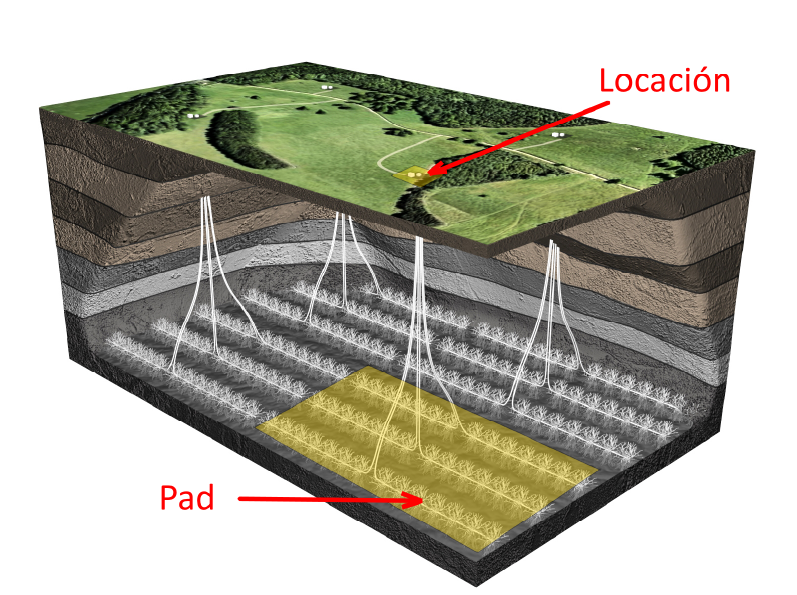
\includegraphics[width=0.15\textwidth]{imagenes/figura2}
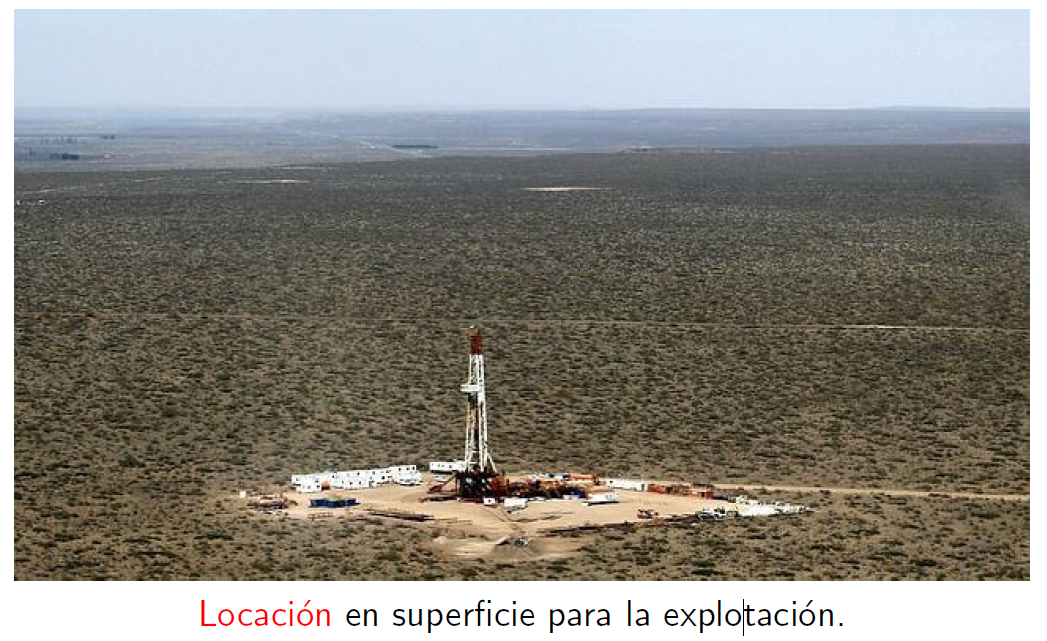
\includegraphics[width=0.15\textwidth]{imagenes/figura3}
\end{center}

Cada perforacion atraviesa la roca madre, y a lo largo de esta perforacion
se realizan los procesos de inyeccion de materiales para lograr la fractura de
la roca. Luego, se utilizan las mismas para la extraccion de los hidrocarburos
que migran hacia las zonas de fractura.

La zona
explotada a partir de una locacion se denomina pad, y tiene una forma tpicamente
rectangular.

Dadas estas caracteristicas del problemas queremos que las zonas de fractura en la roca madre no se deban superponer,